\chapter{PRESENTACI�N Y AN�LISIS DE RESULTADOS}
\section{Selecci\'on del movimiento de cada equipo deportivo} \label{res:idMov}
A continuaci\'on se presenta el formulario de registro de movimiento de cada equipo deportivo (ver anexos, Figura \ref{fig:frmWhiteMov}), en ella se describe la informaci\'on del movimiento con el detalle de los pasos que debe realizar para ejecutar dicho movimiento:
\begin{figure}[H]
	\caption{Formulario de movimiento de tenis de mesa}
	\label{fig:frmMovTen}
	\centering
	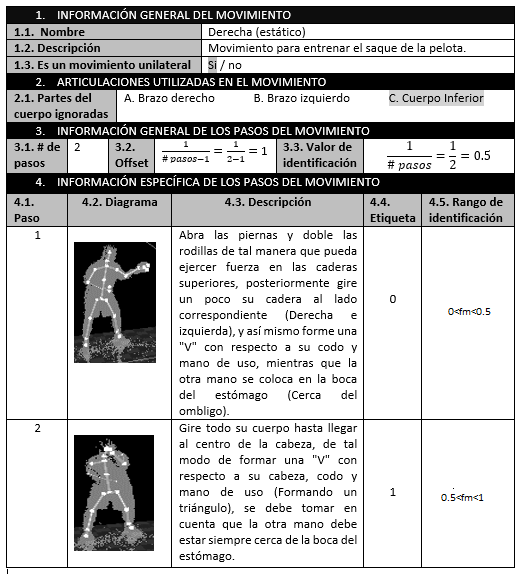
\includegraphics[width=430px,height=330px]{graphics/resultados/movimientoTenis.PNG} \\
	\textbf{Fuente:} Elaborado por el autor de tesis en base a las observaciones del trabajo de campo
\end{figure}
\begin{figure}[H]
	\caption{Formulario de movimiento de animaci\'on}
	\label{fig:frmMovCheer}
	\centering
	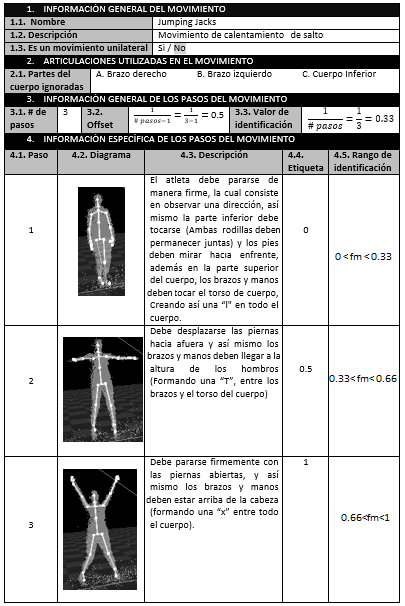
\includegraphics[width=445px,height=600px]{graphics/resultados/movimientoCheerleader.PNG} \\
	\textbf{Fuente:} Elaborado por el autor de tesis en base a las observaciones del trabajo de campo
\end{figure}
\begin{figure}[H]
	\caption{Formulario de movimiento taekwondo}
	\label{fig:frmWhiteMov}
	\centering
	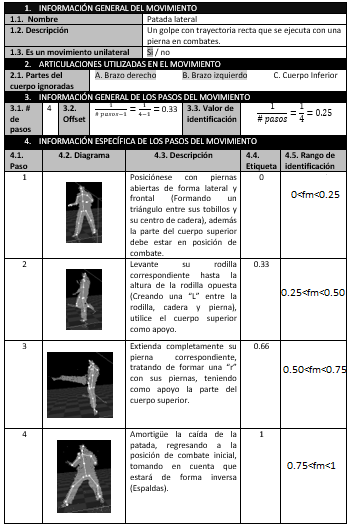
\includegraphics[width=445px,height=600px]{graphics/resultados/movimientoTaekwondo.PNG} \\
	\textbf{Fuente:} Elaborado por el autor de tesis en base a las observaciones del trabajo de campo
\end{figure}
\section{Creaci\'on de rutina del movimiento de cada equipo deportivo} \label{res:idMov}
En esta secci\'on se muestra el formulario de registro de rutina de cada equipo deportivo (ver anexos, figura \ref{fig:frmWhiteRout}), en ella se describe los movimientos de calentamiento que realizaron los atletas previamente al registro de datos (ver anexos, secci\'on \ref{anx:warmup}), detallando el n\'umero de series de repeticiones y el tiempo empleado para realizar todos los movimientos de calentamiento. Finalmente, se muestra la estandarizaci\'on del tipo de rutina que  realizaron cada atleta durante la toma de datos:
\begin{figure}[H]
	\caption{Formulario de rutina de animaci\'on}
	\label{fig:frmRoutCher}
	\centering
	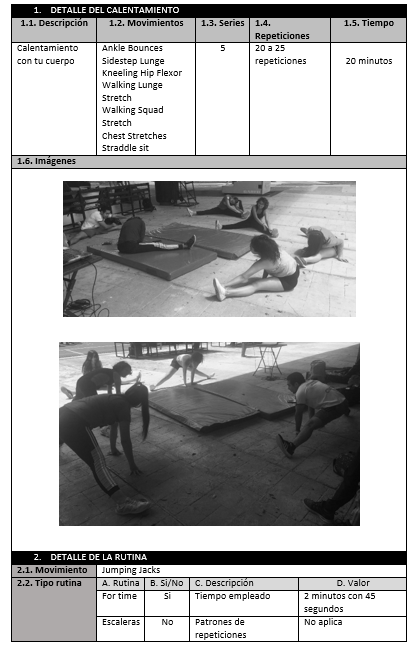
\includegraphics[width=400px,height=490px]{graphics/resultados/rutina-cheerleaders.PNG} \\
	\textbf{Fuente:} Elaborado por el autor de tesis en base a las observaciones del trabajo de campo
\end{figure}
\begin{figure}[H]
	\caption{Formulario de rutina de tenis de mesa}
	\label{fig:frmRoutTen}
	\centering
	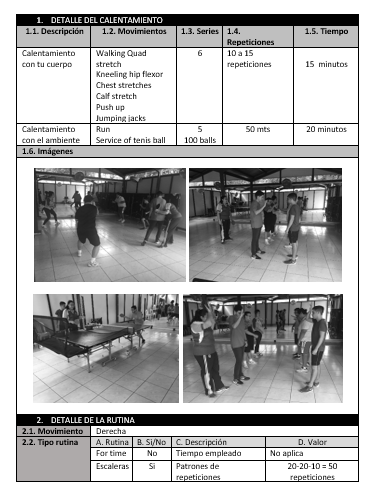
\includegraphics[width=445px,height=600px]{graphics/resultados/rutina-tennis.PNG} \\
	\textbf{Fuente:} Elaborado por el autor de tesis en base a las observaciones del trabajo de campo
\end{figure}
\begin{figure}[H]
	\caption{Formulario de rutina de taekwondo}
	\label{fig:frmRoutTaek}
	\centering
	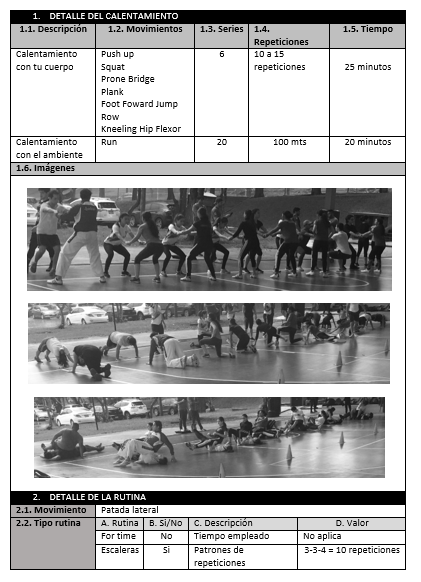
\includegraphics[width=445px,height=600px]{graphics/resultados/rutina-taekwondo.PNG} \\
	\textbf{Fuente:} Elaborado por el autor de tesis en base a las observaciones del trabajo de campo
\end{figure}
\section{Distancias de profundidad recomendadas entre el atleta y el sensor} \label{res:idMov}
En la siguiente tabla se muestra un resumen general de las caracter\'isticas de la poblaci\'on de cada equipo deportivo, en ella se describe la altura promedio y la distancia recomendadas para ejecutar correctamente el seguimiento de esqueleto -i.e. Renderizaci\'on completa del esqueleto humano-, dichos datos fueron capturados por el sensor Kinect a una altura de 0.70 metros desde el suelo y tomando como punto de referencia, la cadera central de cada atleta:
\begin{table}[H]
\begin{center}
\caption{Distancias de profundidad recomendadas para el funcionamiento del seguimiento de esqueleto}
\label{tab:depthCalculation}
\begin{tabular}{lllll}
\hline
\multicolumn{3}{|c|}{Caracter\'isticas generales} & \multicolumn{2}{l|}{\begin{tabular}[c]{@{}l@{}}Distancia de profundidad\\ recomendada entre el \\ usuario y el sensor\end{tabular}} \\ \hline
\multicolumn{1}{|l|}{Deporte} & \multicolumn{1}{l|}{\begin{tabular}[c]{@{}l@{}}Altura promedio\\ (Metros)\end{tabular}} & \multicolumn{1}{l|}{\begin{tabular}[c]{@{}l@{}}Desviaci\'on est\'andar\\ de la altura (metros)\end{tabular}} & \multicolumn{1}{l|}{\begin{tabular}[c]{@{}l@{}}M\'inima\\ (Metros)\end{tabular}} & \multicolumn{1}{l|}{\begin{tabular}[c]{@{}l@{}}M\'axima\\ (Metros)\end{tabular}} \\ \hline
\multicolumn{1}{|l|}{Tenis de mesa} & \multicolumn{1}{l|}{1.302435} & \multicolumn{1}{l|}{0.088683} & \multicolumn{1}{l|}{3.505103} & \multicolumn{1}{l|}{3.990376} \\ \hline
\multicolumn{1}{|l|}{Animaci\'on} & \multicolumn{1}{l|}{1.342471} & \multicolumn{1}{l|}{0.059301} & \multicolumn{1}{l|}{2.763813} & \multicolumn{1}{l|}{3.411942} \\ \hline
\multicolumn{1}{|l|}{Taekwondo} & \multicolumn{1}{l|}{1.373372} & \multicolumn{1}{l|}{0.098490} & \multicolumn{1}{l|}{2.556640} & \multicolumn{1}{l|}{3.869427} \\ \hline
\multicolumn{5}{l}{\textbf{Fuente:} Instrumento \ref{ins:UI:wpf}.\ref{ins:UI:wpf:depth} utilizado en los atletas de construcci\'on y pruebas (ver secci\'on \ref{sj:1t})}
\end{tabular}
\end{center}
\end{table}
\section{Muestras de fotogramas del movimiento} \label{res:fotogramas}
En esta secci\'on se realiz\'o por cada equipo deportivo, un cuadro comparativo, en donde se compara por fotograf\'ias, el seguimiento de esqueleto de cada atleta durante cada paso de una repetici\'on del movimiento. As\'i mismo por cada fotograf\'ia se muestra cuatros elementos importantes:
\begin{itemize}
\item El fondo de color negro.
\item El piso representado por cuadros de colores grises.
\item La figura del atleta figurado por una sombra de color gris.
\item El seguimiento de esqueleto conformado por puntos -i.e. Articulaciones- y lineas de color blanco -i.e. Uni\'on de dos articulaciones-.
\end{itemize}
\begin{figure}[H]
	\caption{Fotogramas de 6 sujetos del equipo de tenis de mesa}
	\label{fig:fotogramaTenis}
	\centering
	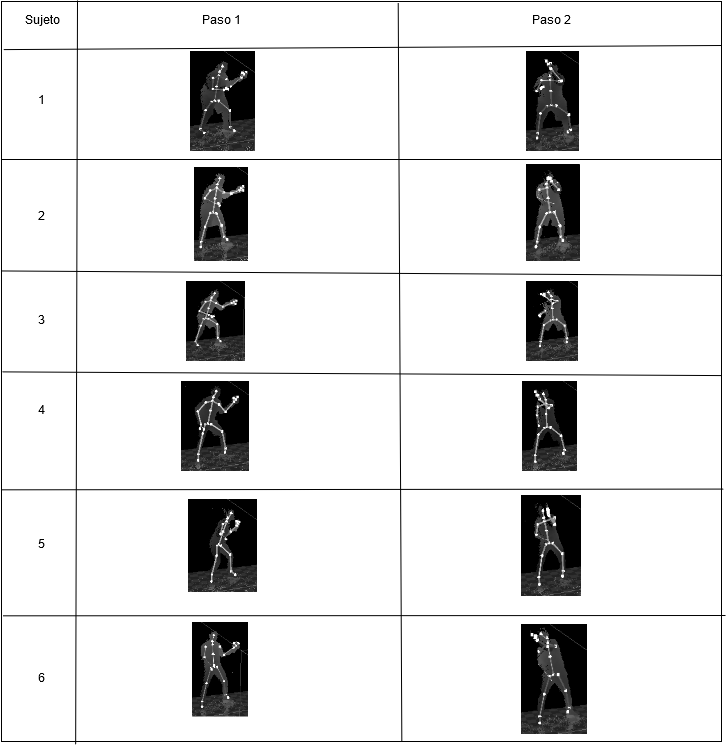
\includegraphics[width=445px,height=600px]{graphics/resultados/SETenisDeMesa.PNG} \\
	\textbf{Fuente:} Recuperado por los v\'ideos de trabajo de campo (ver instrumento \ref{ins:KinectStudio})
\end{figure}
\begin{figure}[H]
	\caption{Fotogramas de 7 sujetos del equipo de animaci\'on}
	\label{fig:fotogramaCheerleader}
	\centering
	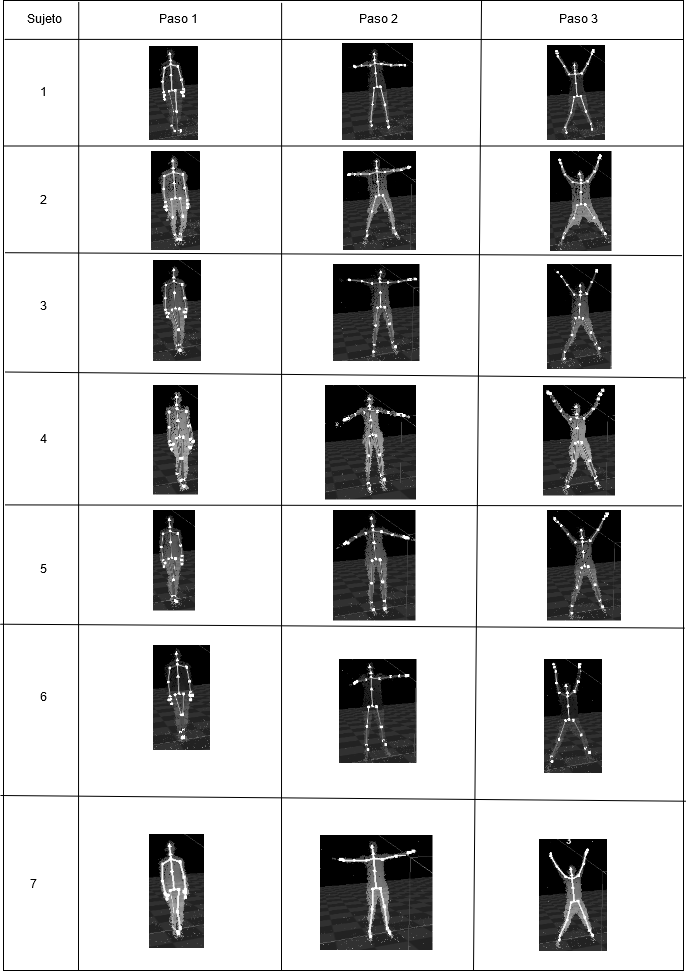
\includegraphics[width=445px,height=600px]{graphics/resultados/SECheerleaders.PNG} \\
	\textbf{Fuente:} Recuperado por los v\'ideos de trabajo de campo (ver instrumento \ref{ins:KinectStudio})
\end{figure}
\begin{figure}[H]
	\caption{Fotogramas de 7 sujetos del equipo de taekwondo}
	\label{fig:fotogramaTaekwondo}
	\centering
	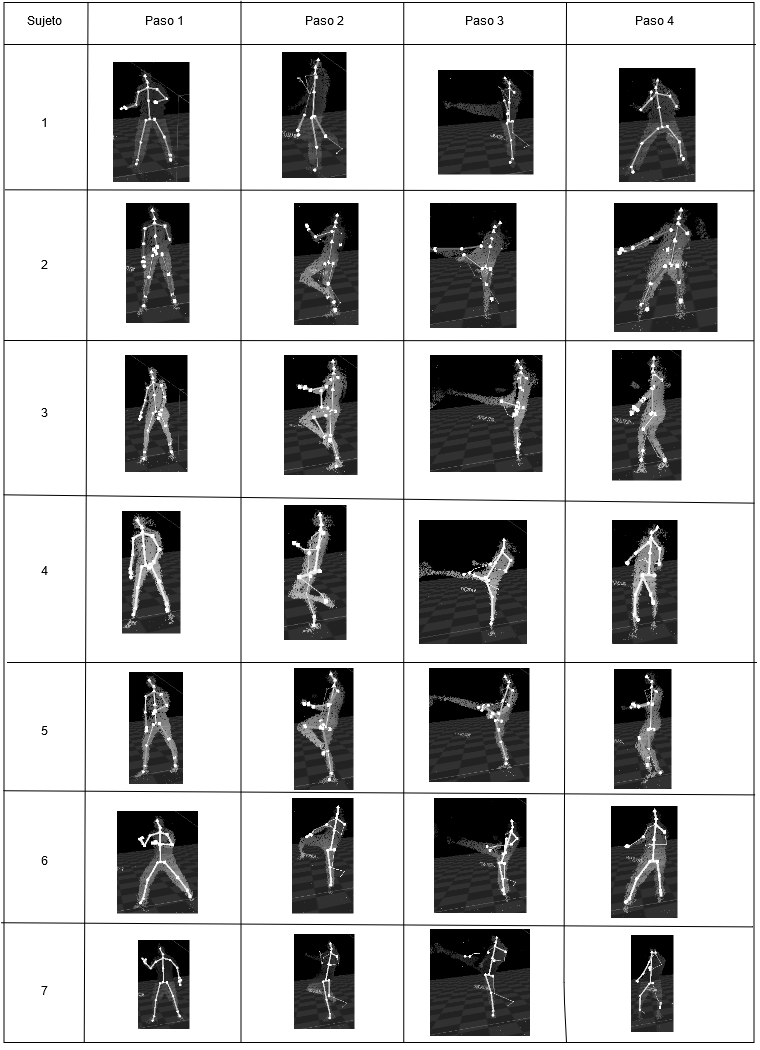
\includegraphics[width=445px,height=600px]{graphics/resultados/SETaekwondo.PNG} \\
	\textbf{Fuente:} Recuperado por los v\'ideos de trabajo de campo (ver instrumento \ref{ins:KinectStudio})
\end{figure}
\begin{landscape}
\section{Razones de fallo del seguimiento de esqueleto}
El seguimiento de esqueleto es unos elementos fundamentales para crear el modelo de reconocimiento de movimiento, sin embargo se debe tomar en cuenta que puede fallar por varias razones, entre ellas se encuentra las siguientes fallas: del atleta -i.e. Hombre-, del sensor Kinect -i.e. M\'aquina-, del lugar de trabajo -i.e. Entorno-, de la interacci\'on  con objetos o elementos externos -i.e. Material-, de la preparaci\'on necesaria para realizar una rutina -i.e. M\'etodo- y finalmente el 
\'area de trabajo para la captura de datos -i.e. Medida-:  
\begin{figure}[H]
	\caption{diagrama de Ishikawa sobre el fallo del seguimiento de esqueleto}
	\label{fig:ishikawa}
	\centering
	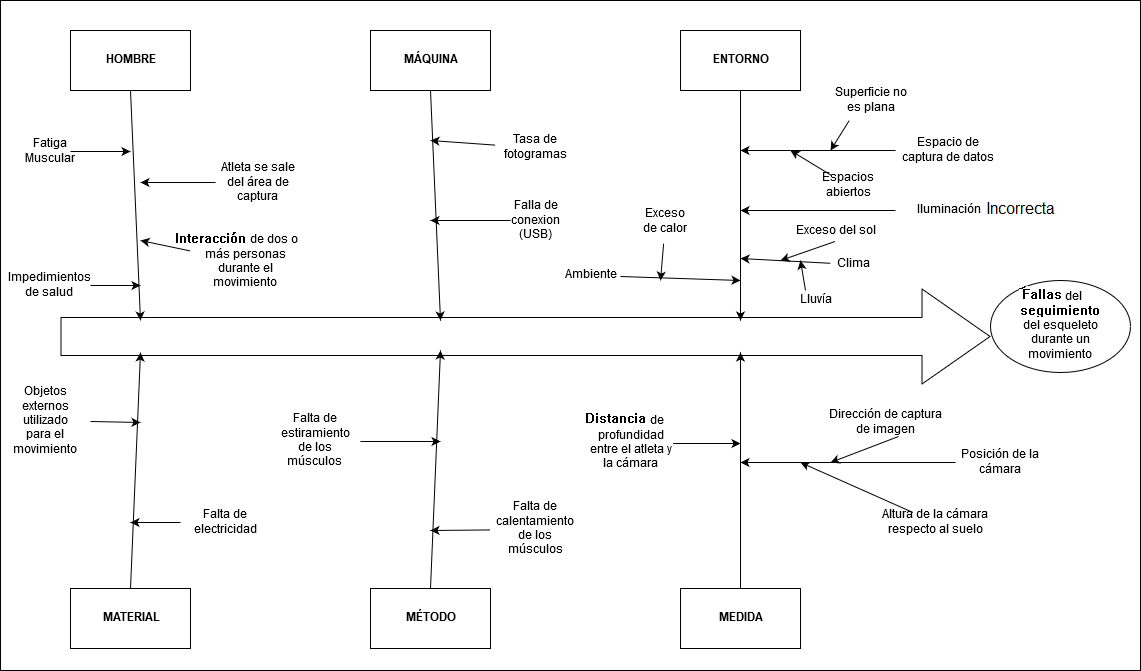
\includegraphics[width=560px,height=330px]{graphics/resultados/Ishi-SeguimientoDeEsqueleto.PNG} \\
	\textbf{Fuente:} Realizado en base a las observaciones de trabajo de campo.
\end{figure}
\end{landscape}
\section{Proceso de etiquetaci\'on de un movimiento}
Consta de un conjunto de gr\'aficas de etiquetaci\'on que se utilizaron para el entrenamiento y testeo del modelo de reconocimiento de un  movimiento, cabe mencionar que por cada gr\'afica se encuentra los siguientes elementos:
\begin{itemize}
\item Una L\'inea recta -i.e. Lectura del fotograma del valor actual-.
\item Una l\'inea curvada que unifica 2 o m\'as puntos -i.e. Representaci\'on de una repetici\'on que pasa por cada paso del movimiento-.
\item Espacios de color gris -i.e. Ruidos o datos basura que no se utilizaron en el proceso de etiquetaci\'on-.
\end{itemize}
Por otro lado se observa que por cada linea curvada, el valor del factor movimiento -i.e. Eje vertical- va aumentado (comenzando con un valor de 0 y finalizando con un valor de 1) por cada fotograma que avanza -i.e. Eje horizontal-, y as\'i mismo se contabiliza todas las lineas curvada para obtener la cantidades de repeticiones totales que se utilizaron para construir y probar el modelo: 
\begin{chart}[H]
	\caption{Etiquetaci\'on de fotogramas del equipo de tenis de mesa}
	\label{fig:etiquetaTenis}
	\centering
	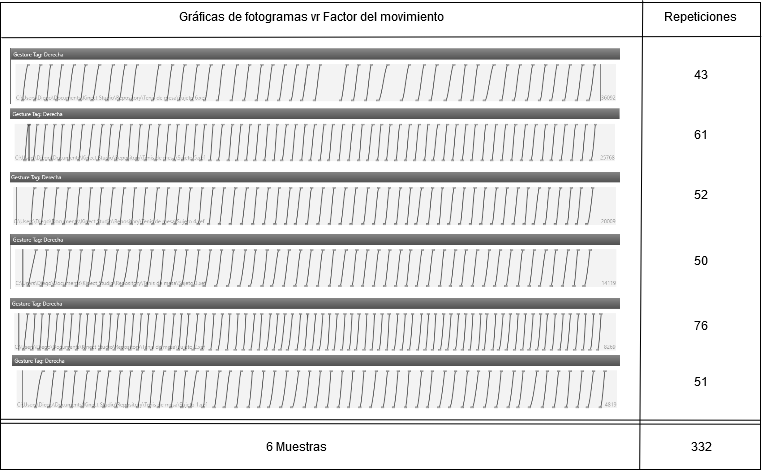
\includegraphics[width=445px,height=260px]{graphics/resultados/GraSegTenisDeMesa.PNG} \\
	\textbf{Fuente:} Recuperado por los v\'ideos etiquetados del trabajo de campo (ver instrumento \ref{ins:VisualGestureBuilder})
\end{chart}
\begin{chart}[H]
	\caption{Etiquetaci\'on de fotogramas del equipo de animaci\'on}
	\label{fig:etiquetaCheerleader}
	\centering
	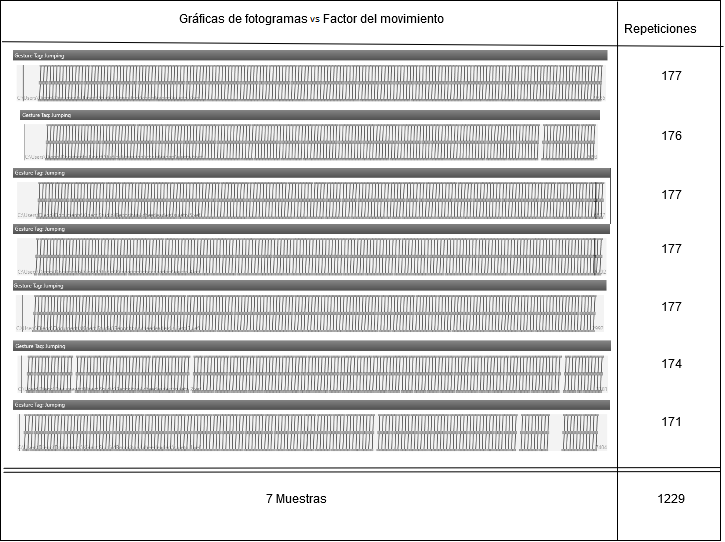
\includegraphics[width=445px,height=220px]{graphics/resultados/GraSegCheerleaders.PNG} \\
	\textbf{Fuente:} Recuperado por los v\'ideos etiquetados del trabajo de campo (ver instrumento \ref{ins:VisualGestureBuilder})
\end{chart}
\begin{chart}[H]
	\caption{Etiquetaci\'on de fotogramas del equipo de taekwondo}
	\label{fig:etiquetaTaekwondo}
	\centering
	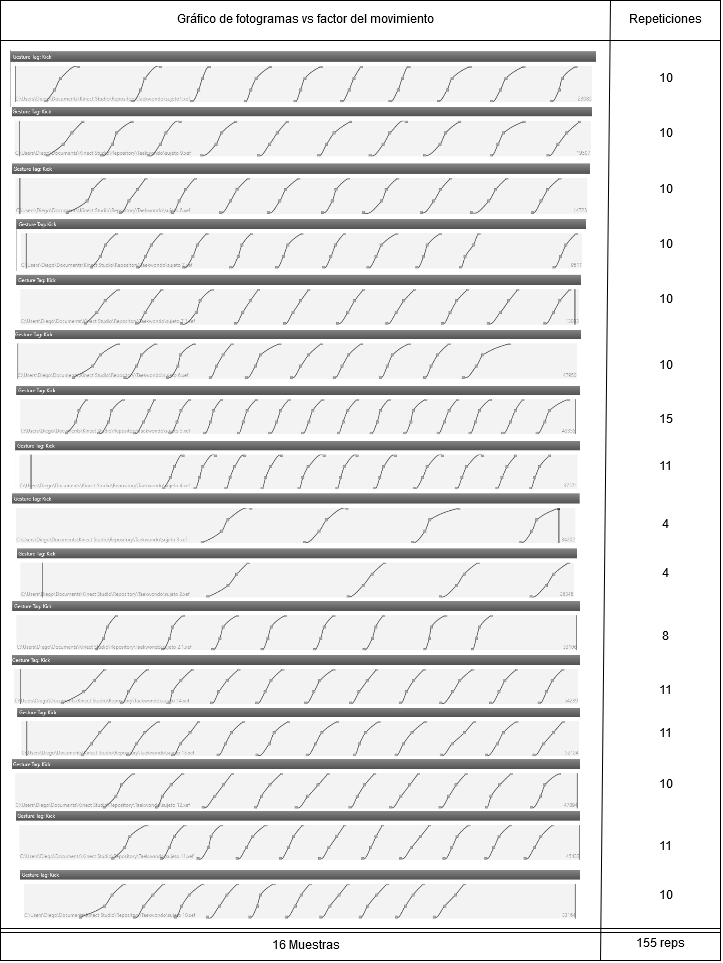
\includegraphics[width=445px,height=350px]{graphics/resultados/GraSegTaekwondo.PNG} \\
	\textbf{Fuente:} Recuperado por los v\'ideos etiquetados del trabajo de campo (ver instrumento \ref{ins:VisualGestureBuilder})
\end{chart}
\section{Selecci\'on y pruebas del modelo} \label{res:chooseModel}
Por cada equipo deportivo se realiz\'o una tabla de informaci\'on del modelo de reconocimiento de un movimiento, la cual se divide en tres partes:
\begin{itemize}
\item  La primera parte se encontr\'o los errores de cada modelo -e.g. Error medio pron\'osticado, desviaci\'on media absoluta y la ra\'iz del error cuadr\'atico medio- y posteriormente se calcul\'o la media de cada error, la cual representa el error de toda la muestra de un equipo deportivo.
\item  La segunda parte se compone en la selecci\'on del modelo que tenga el menor RECM, adem\'as de la aprobaci\'on o el rechazo de cada modelo, dependiendo del valor de identificaci\'on (ver secci\'on \ref{res:idMov}) y el RECM promedio de cada movimiento, as\'i mismo se encontr\'o el factor de reconocimiento  -i.e. Valor n\'umerico que representa la proporcionalidad del valor de identificaci\'on-.
\item Finalmente, la tercera parte se muestra en caso que se apruebe el modelo, la cual detalla los intervalos de confianza de cada modelo -i.e. Intervalo que permite identificar el paso de un movimiento a partir del factor de movimiento-.
\end{itemize}
\begin{table}[H]
\begin{center}
\caption{Modelos y pruebas del equipo de Taekwondo}
\label{tab:chooseTaekwondo}
\begin{tabular}{cccc}
\hline
\multicolumn{4}{|c|}{1. Datos de los errores de los modelos} \\ \hline
\multicolumn{1}{|c|}{\textbf{Modelo}} & \multicolumn{1}{c|}{\textbf{EMP}} & \multicolumn{1}{c|}{\textbf{DMA}} & \multicolumn{1}{c|}{\textbf{RECM}} \\ \hline
\multicolumn{1}{|c|}{1} & \multicolumn{1}{c|}{-0,03543} & \multicolumn{1}{c|}{0,301911} & \multicolumn{1}{c|}{0,374544078} \\ \hline
\multicolumn{1}{|c|}{2} & \multicolumn{1}{c|}{0,050888} & \multicolumn{1}{c|}{0,297433} & \multicolumn{1}{c|}{0,393153} \\ \hline
\multicolumn{1}{|c|}{3} & \multicolumn{1}{c|}{0,200827} & \multicolumn{1}{c|}{0,214594} & \multicolumn{1}{c|}{0,191583} \\ \hline
\multicolumn{1}{|c|}{\textbf{Promedio}} & \multicolumn{1}{c|}{0,072095} & \multicolumn{1}{c|}{0,271313} & \multicolumn{1}{c|}{0,31976} \\ \hline
\multicolumn{1}{l}{} & \multicolumn{1}{l}{} & \multicolumn{1}{l}{} & \multicolumn{1}{l}{} \\ \hline
\multicolumn{4}{|c|}{2. Detalle del modelo} \\ \hline
\multicolumn{3}{|c|}{\textbf{Mejor modelo}} & \multicolumn{1}{c|}{3} \\ \hline
\multicolumn{3}{|c|}{\textbf{Aprueba o rechaza el modelo}} & \multicolumn{1}{c|}{\begin{tabular}[c]{@{}c@{}}Rechaza\\ 0,31976  \textgreater{}= 0.25\end{tabular}} \\ \hline
\multicolumn{3}{|c|}{\textbf{Recognition}} & \multicolumn{1}{c|}{1,27904} \\ \hline
\multicolumn{4}{l}{\textbf{Fuente:} c\'alculo de intervalos de confianza (ver f\'ormula \ref{frm:rangoConfiabilidad})}
\end{tabular}
\end{center}
\end{table}
\begin{table}[H]
\begin{center}
\caption{Modelos y pruebas del equipo de tenis de mesa }
\label{tab:chooseModelTenis}
\begin{tabular}{cccc}
\hline
\multicolumn{4}{|c|}{1. Datos de los errores de los modelos} \\ \hline
\multicolumn{1}{|c|}{\textbf{Modelo}} & \multicolumn{1}{c|}{\textbf{EMP}} & \multicolumn{1}{c|}{\textbf{DMA}} & \multicolumn{1}{c|}{\textbf{RECM}} \\ \hline
\multicolumn{1}{|c|}{1} & \multicolumn{1}{c|}{0,175144} & \multicolumn{1}{c|}{0,217553} & \multicolumn{1}{c|}{0,236069} \\ \hline
\multicolumn{1}{|c|}{2} & \multicolumn{1}{c|}{0,022738} & \multicolumn{1}{c|}{0,113367} & \multicolumn{1}{c|}{0,140393} \\ \hline
\multicolumn{1}{|c|}{3} & \multicolumn{1}{c|}{0,139513} & \multicolumn{1}{c|}{0,260699} & \multicolumn{1}{c|}{0,342375} \\ \hline
\multicolumn{1}{|c|}{\textbf{Promedio}} & \multicolumn{1}{c|}{0,112465} & \multicolumn{1}{c|}{0,197206} & \multicolumn{1}{c|}{0,239612} \\ \hline
\multicolumn{1}{l}{} & \multicolumn{1}{l}{} & \multicolumn{1}{l}{} & \multicolumn{1}{l}{} \\ \hline
\multicolumn{4}{|c|}{2. Detalle del modelo} \\ \hline
\multicolumn{3}{|c|}{\textbf{Mejor modelo}} & \multicolumn{1}{c|}{2} \\ \hline
\multicolumn{3}{|c|}{\textbf{Aprueba o rechaza el modelo}} & \multicolumn{1}{c|}{\begin{tabular}[c]{@{}c@{}}Aprueba\\ 0,239612 \textless 0.5\end{tabular}} \\ \hline
\multicolumn{3}{|c|}{\textbf{Recognition}} & \multicolumn{1}{c|}{0,479225} \\ \hline
\multicolumn{1}{l}{} & \multicolumn{1}{l}{} & \multicolumn{1}{l}{} & \multicolumn{1}{l}{} \\ \hline
\multicolumn{4}{|c|}{3. Detalle del paso del movimiento} \\ \hline
\multicolumn{2}{|c|}{\textbf{Detallle}} & \multicolumn{2}{c|}{\textbf{Intervalo de confianza}} \\ \hline
\multicolumn{1}{|c|}{Paso} & \multicolumn{1}{c|}{Etiqueta} & \multicolumn{1}{c|}{Inferior} & \multicolumn{1}{c|}{Superior} \\ \hline
\multicolumn{1}{|c|}{1} & \multicolumn{1}{c|}{0} & \multicolumn{1}{c|}{0} & \multicolumn{1}{c|}{0,239612} \\ \hline
\multicolumn{1}{|c|}{2} & \multicolumn{1}{c|}{1} & \multicolumn{1}{c|}{0,760388} & \multicolumn{1}{c|}{1} \\ \hline
\multicolumn{4}{l}{\textbf{Fuente:} c\'alculo de intervalos de confianza (ver f\'ormula \ref{frm:rangoConfiabilidad})}
\end{tabular}
\end{center}
\end{table}
\begin{table}[H]
\begin{center}
\caption{Modelos y pruebas del equipo de animaci\'on}
\label{tab:chooseCheerleader}
\begin{tabular}{cccc}
\hline
\multicolumn{4}{|c|}{1. Datos de los errores de los modelos} \\ \hline
\multicolumn{1}{|c|}{\textbf{Modelo}} & \multicolumn{1}{c|}{\textbf{EMP}} & \multicolumn{1}{c|}{\textbf{DMA}} & \multicolumn{1}{c|}{\textbf{RECM}} \\ \hline
\multicolumn{1}{|c|}{1} & \multicolumn{1}{c|}{0,02323} & \multicolumn{1}{c|}{0,038519} & \multicolumn{1}{c|}{0,046957} \\ \hline
\multicolumn{1}{|c|}{2} & \multicolumn{1}{c|}{0,080008} & \multicolumn{1}{c|}{0,083864} & \multicolumn{1}{c|}{0,076391} \\ \hline
\multicolumn{1}{|c|}{3} & \multicolumn{1}{c|}{0,032244} & \multicolumn{1}{c|}{0,04105} & \multicolumn{1}{c|}{0,045347} \\ \hline
\multicolumn{1}{|c|}{\textbf{Promedio}} & \multicolumn{1}{c|}{0,045161} & \multicolumn{1}{c|}{0,054478} & \multicolumn{1}{c|}{0,056232} \\ \hline
\multicolumn{1}{l}{} & \multicolumn{1}{l}{} & \multicolumn{1}{l}{} & \multicolumn{1}{l}{} \\ \hline
\multicolumn{4}{|c|}{2. Detalle del modelo} \\ \hline
\multicolumn{3}{|c|}{\textbf{Mejor modelo}} & \multicolumn{1}{c|}{3} \\ \hline
\multicolumn{3}{|c|}{\textbf{Aprueba o rechaza el modelo}} & \multicolumn{1}{c|}{\begin{tabular}[c]{@{}c@{}}Aprueba\\ 0,056232 \textless 0.33\end{tabular}} \\ \hline
\multicolumn{3}{|c|}{\textbf{Recognition}} & \multicolumn{1}{c|}{0,168695} \\ \hline
\multicolumn{1}{l}{} & \multicolumn{1}{l}{} & \multicolumn{1}{l}{} & \multicolumn{1}{l}{} \\ \hline
\multicolumn{4}{|c|}{3. Detalle del paso del movimiento} \\ \hline
\multicolumn{2}{|c|}{\textbf{Detallle}} & \multicolumn{2}{c|}{\textbf{Intervalo de confianza}} \\ \hline
\multicolumn{1}{|c|}{Paso} & \multicolumn{1}{c|}{Etiqueta} & \multicolumn{1}{c|}{Inferior} & \multicolumn{1}{c|}{Superior} \\ \hline
\multicolumn{1}{|c|}{1} & \multicolumn{1}{c|}{0} & \multicolumn{1}{c|}{0} & \multicolumn{1}{c|}{0,056232} \\ \hline
\multicolumn{1}{|c|}{2} & \multicolumn{1}{c|}{0.5} & \multicolumn{1}{c|}{0,471884} & \multicolumn{1}{c|}{0,528116} \\ \hline
\multicolumn{1}{|c|}{3} & \multicolumn{1}{c|}{1} & \multicolumn{1}{c|}{0,943768} & \multicolumn{1}{c|}{1} \\ \hline
\multicolumn{4}{l}{\textbf{Fuente:} c\'alculo de intervalos de confianza (ver f\'ormula \ref{frm:rangoConfiabilidad})}
\end{tabular}
\end{center}
\end{table}
\section{Muestra de regresiones de los movimiento} \label{res:regretions}
Estos resultados demuestra un ejemplo de las posibles regresiones que puede implementar el modelo de machine learning -i.e. Random Forest Regression-, adem\'as de comprobar que los modelos aceptados fueron entrenados con distintos datos de entrenamientos (Uniformidad con los tiempo de capturas y una dispersi\'on con los recorridos de una articulaci\'on, durante la ejecuci\'on del  movimiento).
\begin{figure}[H]
	\caption{Regresi\'on distancia vs tiempo, del equipo animaci\'on}
	\label{fig:regrCheerleader}
	\centering
	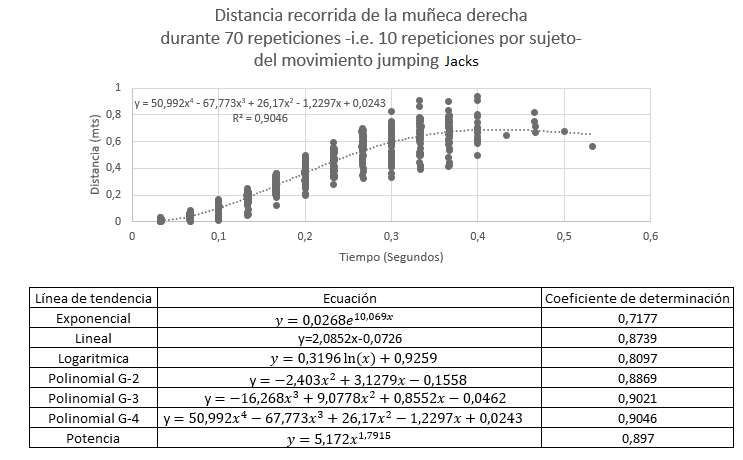
\includegraphics[width=445px,height=200px]{graphics/resultados/cluster-cheerleaders.PNG} \\
	\textbf{Fuente:} Recuperado por los v\'ideos etiquetados del trabajo de campo (ver secci\'on \ref{dis:even})
\end{figure}
\begin{figure}[H]
	\caption{Regresi\'on distancia vs tiempo, del equipo de tenis de mesa}
	\label{fig:regrTennisDeMesa}
	\centering
	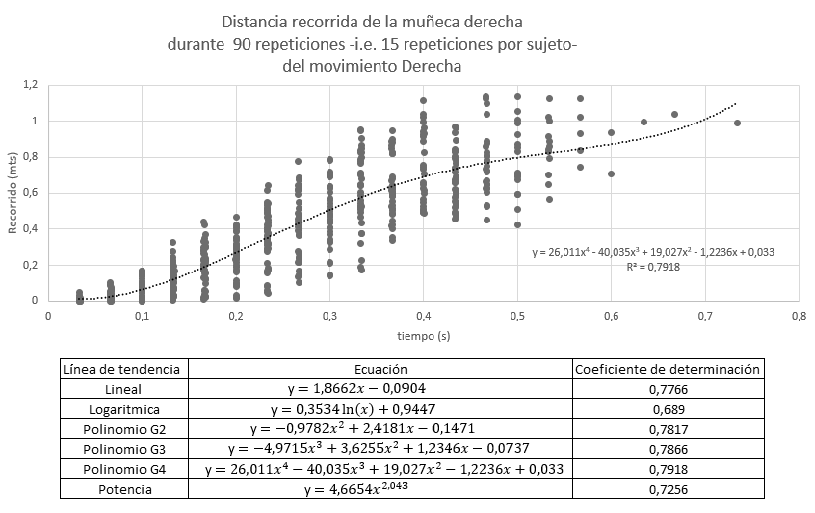
\includegraphics[width=445px,height=200px]{graphics/resultados/cluster-tennis.PNG} \\
	\textbf{Fuente:} Recuperado por los v\'ideos etiquetados del trabajo de campo (ver secci\'on \ref{dis:even})
\end{figure}
\section{Reconocimiento de movimiento}
En esta secci\'on se ense\~na los resultados de la interfaz gr\'afica del reconocimiento de repeticiones de un movimiento, la cual esta conformado por un conjunto de im\'agenes que muestran el seguimiento de esqueleto durante la ejecuci\'on de una repetici\'on, as\'i mismo en cada imagen se muestran los siguientes detalles:
\begin{itemize}
\item \textbf{Estado:} Tiene el valor de TRABAJO, debido que fue capturado durante el tiempo de trabajo en una rutina de tabata.
\item \textbf{Temporizador:} Tiempo de cuenta regresiva, la cual indica cu\'antos segundos le queda al atleta en el estado de trabajo.
\item \textbf{Serie:} Le indica al atleta, cu\'al n\'umero de serie se esta ejecutando (Los resultados fueron capturado durante la serie \# 1 de trabajo).
\item \textbf{Repeticiones:} Le muestra al atleta la cantidad de repeticiones que lleva durante las  series de trabajo (Se debe observar que este indicador incrementa en el \'ultimo paso de cada movimiento).
\item \textbf{Paso:} N\'umero que indica el \'ultimo paso ejecutado (Comenzando desde el valor 0). Se debe tomar en cuenta que dicho valor cambia dependiendo del factor de movimiento -i.e. Progreso-, es decir reconoce cada paso del movimiento, ya que el valor del progreso se encuentra dentro de alg\'un intervalo de confianza (Ver secci\'on \ref{res:chooseModel}).
\item \textbf{Progreso:} Factor del movimiento en tiempo real (Obtenido a partir de la base de datos de gesturas), la cual va incrementado por cada paso que avance el atleta.
\item \textbf{Tiempo Total:} Tiempo total que lleva actualmente el atleta (En los resultados se puede ver que el atleta emplea una repetici\'on en un per\'iodo de d\'ecimas de segundos).
\end{itemize}
\begin{figure}[H]
	\caption{Reconocimiento del movimiento Derecha}
	\label{fig:recognitionTenis}
	\centering
	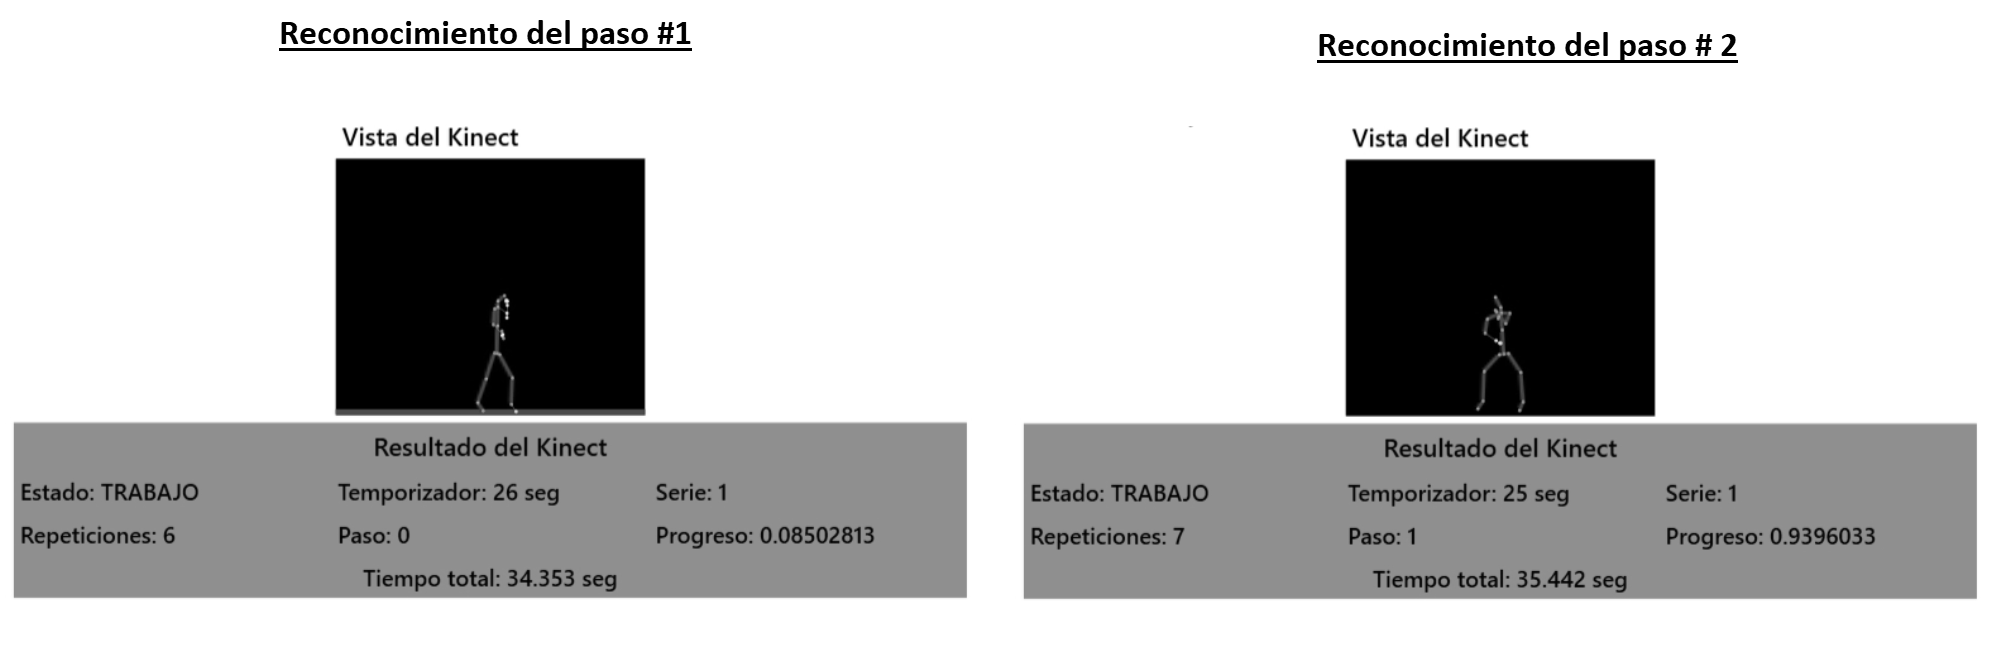
\includegraphics[width=420px,height=250px]{graphics/resultados/recognitionTennis.png} \\
	\textbf{Fuente:} sujeto de validaci\'on del modelo en tiempo real (Ver instrumento \ref{ins:UI:wpf}.\ref{ins:UI:wpf:evaluate})
\end{figure}
\begin{figure}[H]
	\caption{Reconocimiento del movimiento Jumping Jacks}
	\label{fig:recognitionCheerleader}
	\centering
	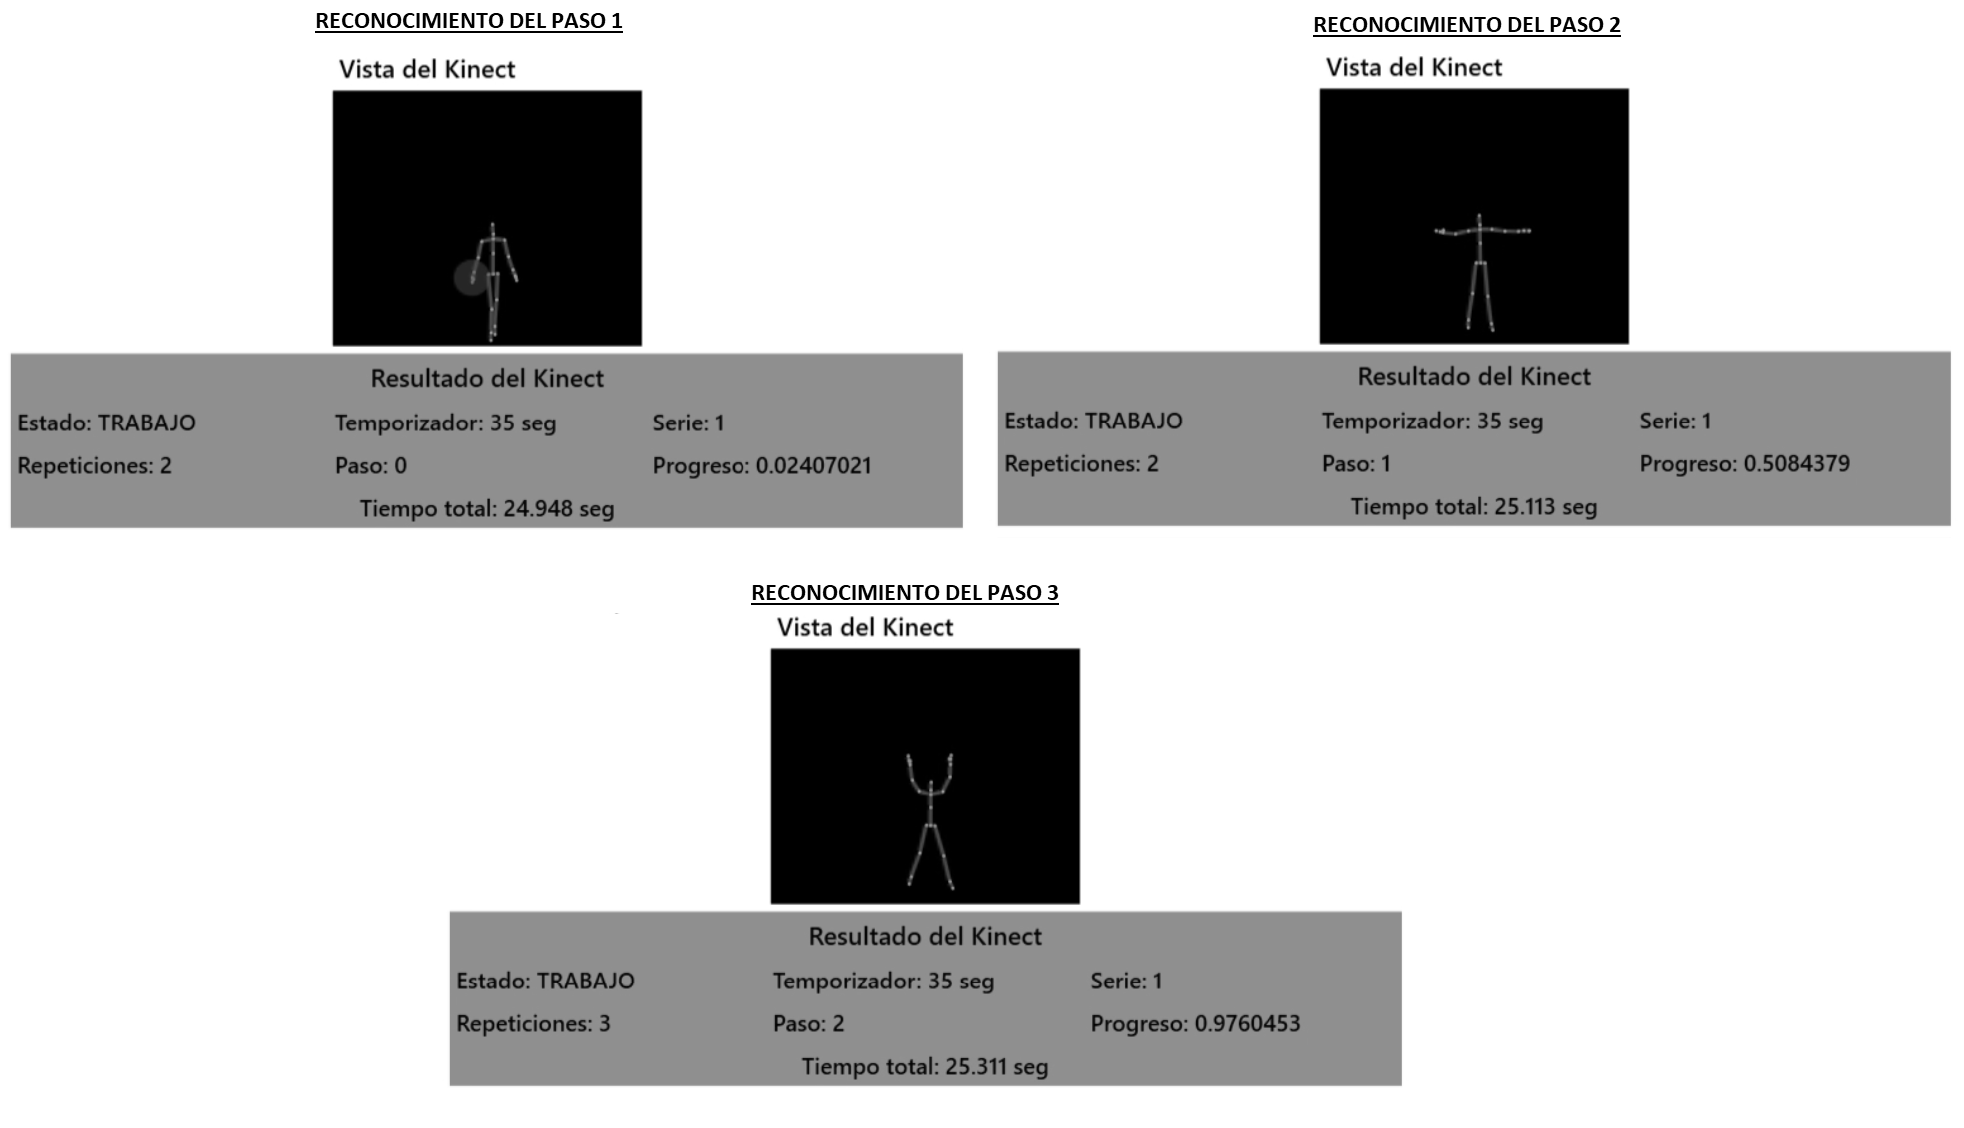
\includegraphics[width=430px,height=320px]{graphics/resultados/recognitionCheerleader.png} \\
	\textbf{Fuente:} sujeto de validaci\'on del modelo en tiempo real (Ver instrumento \ref{ins:UI:wpf}.\ref{ins:UI:wpf:evaluate})
\end{figure}
\section{Validaci\'on del movimiento} \label{res:valResults}
A continuaci\'on se presenta la interfaz gr\'afica de los resultados de la rutina tabata por equipo deportivo, se debe considerar que para estos resultados se utiliz\'o atletas que no participaron en la toma de datos iniciales -i.e. Construcci\'on y testeo del modelo-, adem\'as de interpretar en dos partes los elementos del archivo de resultados de una rutina tabata (Ver anexos, c\'odigo \ref{code:tabata}):
\begin{itemize}
\item La primera parte consta de un conjunto de gr\'aficas que muestra de manera visual, el esfuerzo -i.e. Endurance- de cada atleta durante la rutina Tabata.
\item La segunda parte es un cuadro que detalla el  resumen ejecutivo de los resultados de la rutina tabata.
\end{itemize}
\begin{landscape}
\begin{chart}[H]
	\caption{Resultados del tabata del equipo de tenis de mesa}
	\label{fig:resTabTennis}
	\centering
	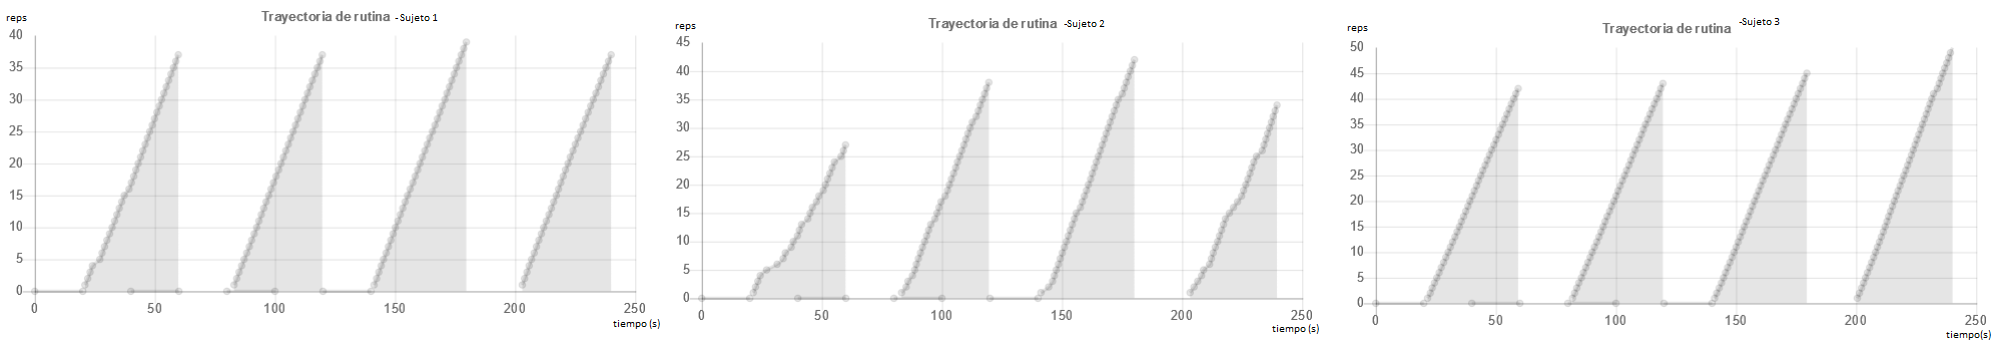
\includegraphics[width=610px,height=200px]{graphics/resultados/ResultRecognitionTenis.png} \\
	\textbf{Fuente:} Realizado en base a las observaciones de trabajo de campo (Ver instrumento \ref{ins:UI:web}.\ref{ins:UI:web:result}).
\end{chart}
\begin{table}[H]
\begin{center}
\caption{Detalle de la rutina tabata del equipo de tenis de mesa}
\label{tab:detailResultsTennis}
\begin{tabular}{|l|l|l|l|l|l|l|l|l|l|}
\hline
\textbf{Series} & \textbf{\begin{tabular}[c]{@{}l@{}}Trabajo\\ (segs)\end{tabular}} & \textbf{\begin{tabular}[c]{@{}l@{}}Descanso\\ (segs)\end{tabular}} & \textbf{\begin{tabular}[c]{@{}l@{}}Duraci\'on\\ (segs)\end{tabular}} & \textbf{Sujeto} & \textbf{\begin{tabular}[c]{@{}l@{}}Volumen de\\ repeticiones\end{tabular}} & \textbf{\begin{tabular}[c]{@{}l@{}}Repeticiones\\ M\'aximas en una\\ serie\end{tabular}} & \textbf{\begin{tabular}[c]{@{}l@{}}Tiempo m\'inimo\\ en una serie\\ (segs)\end{tabular}} & \textbf{\begin{tabular}[c]{@{}l@{}}Repeticiones \\ promedio por\\ serie\end{tabular}} & \textbf{\begin{tabular}[c]{@{}l@{}}Tiempo \\ promedio por\\ repetici\'on (segs)\end{tabular}} \\ \hline
\multirow{3}{*}{4} & \multirow{3}{*}{40} & \multirow{3}{*}{20} & \multirow{3}{*}{240} & 1 & 150 & 39 & 38.5440 & 38 & 0.7106 \\ \cline{5-10} 
 &  &  &  & 2 & 141 & 42 & 39.1050 & 35 & 0.7869 \\ \cline{5-10} 
 &  &  &  & 3 & 180 & 50 & 39.7980 & 45 & 0.3599 \\ \hline
 \multicolumn{10}{l}{\textbf{Fuente:} gr\'afica \ref{fig:resTabTennis}}
\end{tabular}
\end{center}
\end{table}
\begin{chart}[H]
	\caption{Resultados del tabata del equipo de animaci\'on}
	\label{fig:resTabCheerleader}
	\centering
	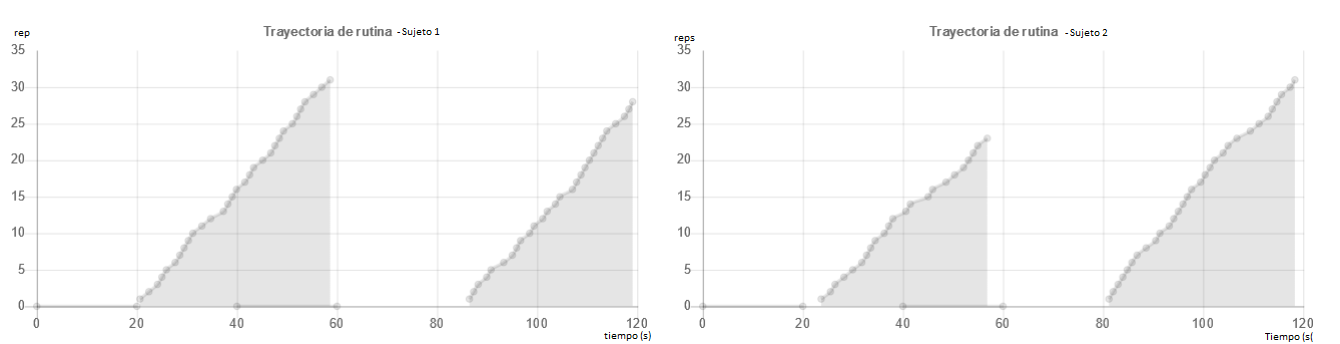
\includegraphics[width=610px,height=200px]{graphics/resultados/ResultRecognitionCheerleader.png} \\
	\textbf{Fuente:} Realizado en base a las observaciones de trabajo de campo (Ver instrumento \ref{ins:UI:web}.\ref{ins:UI:web:result}).
\end{chart}
\begin{table}[H]
\begin{center}
\caption{Detalle de la rutina tabata del equipo de animaci\'on}
\label{tab:detailResultsCheerleader}
\begin{tabular}{|l|l|l|l|l|l|l|l|l|l|}
\hline
\textbf{Series} & \textbf{\begin{tabular}[c]{@{}l@{}}Trabajo\\ (segs)\end{tabular}} & \textbf{\begin{tabular}[c]{@{}l@{}}Descanso\\ (segs)\end{tabular}} & \textbf{\begin{tabular}[c]{@{}l@{}}Duraci\'on\\ (segs)\end{tabular}} & \textbf{Sujeto} & \textbf{\begin{tabular}[c]{@{}l@{}}Volumen de\\ repeticiones\end{tabular}} & \textbf{\begin{tabular}[c]{@{}l@{}}Repeticiones\\ M\'aximas en una\\ serie\end{tabular}} & \textbf{\begin{tabular}[c]{@{}l@{}}Tiempo m\'inimo\\ en una serie\\ (segs)\end{tabular}} & \textbf{\begin{tabular}[c]{@{}l@{}}Repeticiones \\ promedio por\\ serie\end{tabular}} & \textbf{\begin{tabular}[c]{@{}l@{}}Tiempo \\ promedio por\\ repetici\'on (segs)\end{tabular}} \\ \hline
\multirow{2}{*}{2} & \multirow{2}{*}{40} & \multirow{2}{*}{20} & \multirow{2}{*}{120} & 1 & 59 & 31 & 38.3130 & 30 & 0.8284 \\ \cline{5-10} 
 &  &  &  & 2 & 54 & 31 & 37.5210 & 27 & 0.9301 \\ \hline
 \multicolumn{10}{l}{\textbf{Fuente} gr\'afica \ref{fig:resTabCheerleader}}
\end{tabular}
\end{center}
\end{table}
\end{landscape}